\newpage
\pagestyle{fancy}
\lhead{\textsc{Chapitre 1. Étude préalable}}
\renewcommand{\headrulewidth}{0.5pt}
\renewcommand{\footrulewidth}{0.5pt}
\chapter{Étude préalable}\setlength{\headheight}{28pt}
\label{ch1}
\thispagestyle{empty}
\minitoc
\newpage

\section{Introduction}

Ce premier chapitre pose les bases du projet en présentant l'organisme d'accueil, le cadre du stage,
l'analyse de l'existant, la problématique identifiée et la solution proposée. Il constitue le fondement
sur lequel repose l'ensemble des décisions de conception et de développement.

% ─────────────────────────────────────────────────────────────────────────────
\section{Présentation de l'organisme d'accueil}

\subsection{Historique}

EDI SOLUTIONS est une entreprise spécialisée dans les services d'ingénierie informatique et les
solutions digitales. Elle a été créée pour aider les entreprises à se transformer numériquement en
développant des solutions adaptées à leurs besoins. Au fil du temps, elle a élargi ses activités pour
inclure le développement web, l'intégration de systèmes d'information et les solutions ERP.

\begin{figure}[H]
    \centering
    
\includegraphics[width=0.2\textwidth]{Figures/logo_societe.png}
    \caption{Logo d'EDI SOLUTIONS}
    \label{fig:logo_societe}
\end{figure}

\subsection{Domaine d'activité}

L'entreprise opère principalement dans le secteur des technologies de l'information et de la
communication. Ses activités incluent :

\begin{itemize}
    \item Le conseil et l'audit des systèmes d'information ;
    \item Le développement d'applications web et mobiles ;
    \item L'intégration de solutions ERP et cloud ;
    \item La mise en place de systèmes d'information sur mesure.
\end{itemize}

\subsection{Positionnement}

L'entreprise se positionne comme un fournisseur de solutions numériques innovantes, capable de répondre
aux besoins spécifiques des entreprises de toutes tailles. Elle se distingue par sa capacité à proposer
des solutions personnalisées et évolutives, adaptées aux processus métiers de ses clients.

\subsection{Produits et services}

Les principaux services proposés incluent :

\begin{itemize}
    \item Développement de solutions web et mobiles.
    \item Mise en place de plateformes de gestion (ERP).
    \item Solutions e-commerce et e-booking.
    \item Audit et optimisation des systèmes d'information.
    \item Accompagnement à la transformation digitale.
\end{itemize}

\subsection{Organisation et environnement de travail}

La structure de l'entreprise est basée sur une approche axée sur les projets, où les groupes
collaborent ensemble. Le milieu de travail repose sur des outils contemporains de création de
logiciels, promouvant des méthodes agiles, en particulier Scrum, ainsi que l'emploi de technologies
web actuelles telles que React et Next.js.

% ─────────────────────────────────────────────────────────────────────────────
\section{Cadre du stage}

\subsection{Type et durée du stage}

Le stage effectué était un stage de fin d'études, réalisé durant la dernière année de licence en
informatique de gestion. Ce stage a duré quatre mois et a inclus les phases d'analyse, de conception,
de développement et de documentation.

\subsection{Missions réalisées}

Durant ce stage, plusieurs missions ont été effectuées :

\begin{itemize}
    \item Analyse des besoins du système de gestion du service après-vente.
    \item Étude de l'existant et identification des limites.
    \item Conception des diagrammes UML (cas d'utilisation, classes, séquences).
    \item Participation à la définition de l'architecture de l'application.
    \item Développement progressif des fonctionnalités selon la méthodologie Scrum.
\end{itemize}

\subsection{Contribution au projet}

La principale contribution a été de concevoir et créer une application web pour la gestion du service
après-vente. Ce projet a permis de structurer les processus de gestion des interventions, d'automatiser
la planification des opérations de maintenance, d'améliorer la traçabilité des interventions et de
contribuer à la modélisation et à la création des divers modules du système.

% ─────────────────────────────────────────────────────────────────────────────
\section{Cadre du projet}

\subsection{Problématique}

La gestion actuelle du service après-vente est affectée par plusieurs problèmes dus à l'absence d'un
système centralisé et automatisé. Cela entraîne des difficultés dans la planification des interventions,
un suivi inefficace des contrats de maintenance, ainsi qu'une confusion entre les interventions
préventives et curatives.

De plus, la facturation des interventions hors contrat est faite manuellement, ce qui augmente le
risque d'erreurs et ralentit le processus global. Le manque de visibilité en temps réel sur les
interventions et les techniciens complique également la prise de décision.

\subsection{Objectifs à atteindre}

L'objectif principal du projet est de concevoir et développer une application web pour digitaliser et
centraliser la gestion du service après-vente afin d'améliorer son efficacité globale. Les objectifs
spécifiques sont :

\begin{itemize}
    \item Centraliser les données clients, équipements et contrats.
    \item Automatiser la planification des interventions préventives à la création des contrats.
    \item Gérer efficacement les interventions curatives et leur traçabilité.
    \item Assurer la traçabilité complète des opérations.
    \item Automatiser la génération des factures pour les interventions hors contrat.
    \item Améliorer la coordination entre les acteurs du système.
    \item Fournir une meilleure visibilité sur l'activité via des tableaux de bord différenciés.
\end{itemize}

% ─────────────────────────────────────────────────────────────────────────────
\section{Analyse de l'existant}

\subsection{Étude de l'existant}

Le service après-vente se base principalement sur la gestion des contrats de maintenance, le suivi des
équipements installés et la réalisation d'interventions techniques. Les informations relatives aux
clients et aux équipements sont généralement enregistrées dans des fichiers bureautiques ou des dossiers
administratifs. Ces informations comprennent les coordonnées du client, le type d'équipement, la
localisation et l'historique des interventions.

Lors de l'installation d'un équipement, un contrat de maintenance peut être établi. Ce contrat précise
la durée du service, la fréquence des visites préventives et les équipements couverts. Les contrats
servent de référence pour planifier les interventions périodiques.

Les interventions préventives sont programmées selon une périodicité définie dans le contrat, en
fonction de l'exigence de la fiche technique de la machine. L'administrateur prépare un planning et
attribue les tâches aux techniciens en fonction de leur disponibilité.

En cas de panne, le client contacte l'entreprise afin de signaler un dysfonctionnement. Une intervention
curative est alors enregistrée et assignée à un technicien. Ces interventions peuvent faire l'objet
d'une facturation lorsqu'elles ne sont pas couvertes par un contrat.

Le technicien effectue l'intervention sur site, réalise le diagnostic, procède à la maintenance ou à
la réparation et valide la fin de l'intervention. Les informations sont ensuite enregistrées et archivées
dans les documents administratifs internes.

Les interventions hors contrat donnent lieu à une facturation basée sur plusieurs critères, notamment :

\begin{itemize}
    \item Le type d'intervention,
    \item Le matériel utilisé,
    \item Le temps de travail.
\end{itemize}

Le fonctionnement actuel du service après-vente s'appuie principalement sur :

\begin{itemize}
    \item Des fichiers tableurs,
    \item Des documents papier,
    \item Des communications téléphoniques,
    \item La messagerie.
\end{itemize}

\subsection{Critiques de l'existant}

\begin{table}[H]
\centering
\caption{Critiques de l'existant}
\label{tab:ch1:critiques}
\begin{tabular}{|p{3.8cm}|p{5.5cm}|p{5.5cm}|}
\hline
\textbf{Aspect étudié} & \textbf{Avantages} & \textbf{Inconvénients} \\
\hline
Gestion des clients et équipements
  & Les informations de base sur les clients et le matériel sont bien conservées.
  & Informations dispersées sur plusieurs supports, ce qui complique leur gestion. \\
\hline
Gestion des contrats
  & Existence d'un suivi des contrats de maintenance.
  & Difficulté de mise à jour et consultation rapide. \\
\hline
Planification des interventions
  & Les visites préventives sont organisées en fonction de leur périodicité.
  & La planification manuelle peut entraîner des oublis. \\
\hline
Gestion des interventions curatives
  & Possibilité d'enregistrer les demandes clients.
  & Manque d'automatisation dans le traitement. \\
\hline
Suivi des interventions
  & Un historique est conservé dans les documents internes.
  & Traçabilité limitée et difficile à exploiter. \\
\hline
Communication entre acteurs
  & Les échanges directs sont rapides.
  & Risque de perte d'informations et coordination complexe. \\
\hline
Facturation
  & Facturation basée sur les interventions réalisées.
  & La génération des factures est manuelle et nécessite beaucoup de temps. \\
\hline
Outils utilisés
  & Simplicité des outils bureautiques.
  & Absence de centralisation et faible intégration. \\
\hline
\end{tabular}
\end{table}

\subsection{Les applications existantes}

\textbf{Application 1 : Odoo Maintenance}

Odoo est un ERP open source qui propose plusieurs modules, notamment pour la gestion de maintenance,
le support client et la facturation.

\textbf{Avantages :}
\begin{itemize}
    \item Gestion des équipements.
    \item Planification des maintenances préventives.
    \item Gestion des tickets.
\end{itemize}

\textbf{Limites :}
\begin{itemize}
    \item Complexité de configuration.
    \item Coût élevé pour certaines fonctionnalités.
    \item Trop généraliste pour des besoins spécifiques.
\end{itemize}

\textbf{Application 2 : Mainti4 (logiciel GMAO)}

\textbf{Avantages :}
\begin{itemize}
    \item Planification automatique.
    \item Historique complet des interventions.
    \item Tableaux de bord analytiques.
\end{itemize}

\textbf{Inconvénients :}
\begin{itemize}
    \item Solution lourde pour PME.
    \item Interface parfois complexe.
    \item Formation nécessaire.
\end{itemize}

\subsection{Analyse SWOT}

\begin{table}[H]
\centering
\caption{Analyse SWOT de la situation actuelle du service après-vente}
\label{tab:ch1:swot}
\begin{tabular}{|p{1.8cm}|p{6.5cm}|p{6.5cm}|}
\hline
 & \textbf{Forces} & \textbf{Faiblesses} \\
\hline
\textbf{Internes}
  & Existence d'un processus SAV structuré ; expérience métier des techniciens ;
    disponibilité d'un historique des interventions ; présence de contrats de maintenance ;
    relation continue avec les clients.
  & Absence d'un système informatisé centralisé ; données dispersées (Excel, papier, appels) ;
    suivi manuel des interventions et contrats ; manque de visibilité en temps réel ;
    risque élevé d'erreurs dans la facturation. \\
\hline
\textbf{Externes}
  & \textbf{Opportunités} : transformation digitale des entreprises ; automatisation des processus
    métier ; amélioration de la productivité ; meilleure exploitation des données.
  & \textbf{Menaces} : résistance au changement des utilisateurs ; risque de perte de données
    existantes ; dépendance aux méthodes manuelles actuelles ; complexité d'adoption du nouveau
    système. \\
\hline
\end{tabular}
\end{table}

L'analyse SWOT de la situation actuelle du service après-vente indique que l'organisation dispose
déjà d'une structure, mais celle-ci manque de modernité. Le système en place s'appuie sur des
techniques éprouvées, telles que la gestion des clients, des équipements et des contrats de
maintenance, ainsi que sur les données relatives aux interventions antérieures. Ces composants sont
essentiels pour établir un système informatique. Toutefois, cette évaluation souligne aussi plusieurs
problèmes majeurs, notamment l'absence de centralisation et le déficit d'automatisation dans les
processus de facturation et de planification.

% ─────────────────────────────────────────────────────────────────────────────
\section{Solution proposée}

Après avoir analysé la situation actuelle et identifié les limites des méthodes de gestion du service
après-vente, il est clair qu'il est nécessaire de mettre en place une solution informatique pour
améliorer l'organisation, le suivi et la coordination des activités de maintenance.

Nous proposons de créer une application web pour la gestion du service après-vente, destinée aux
entreprises qui installent et maintiennent des climatiseurs et des systèmes de surpression. Cette
solution permettra de :

\begin{itemize}
    \item Centraliser les données clients, équipements et contrats ;
    \item Gérer un catalogue global d'équipements et leur affectation aux clients ;
    \item Automatiser la génération du planning des interventions préventives ;
    \item Assurer le suivi complet des interventions curatives et préventives ;
    \item Permettre aux clients de déclarer leurs pannes en ligne ;
    \item Automatiser la facturation des interventions hors contrat ;
    \item Offrir des tableaux de bord différenciés selon le rôle de l'utilisateur.
\end{itemize}

L'application comportera plusieurs modules :

\begin{itemize}
    \item Gestion des utilisateurs internes (administrateur et technicien) ;
    \item Gestion des clients (société ou personne physique) ;
    \item Catalogue d'équipements avec affectation client ;
    \item Gestion des contrats de maintenance ;
    \item Gestion des interventions préventives et curatives ;
    \item Gestion des pannes et pièces jointes ;
    \item Gestion de la facturation ;
    \item Planning et historique ;
    \item Tableaux de bord différenciés par rôle.
\end{itemize}

% ─────────────────────────────────────────────────────────────────────────────
\section{Processus de développement}

\subsection{Les méthodologies Agile}

Les méthodologies agiles sont des approches de gestion de projets de manière flexible. Elles permettent
de s'adapter aux changements, de travailler en équipe et de livrer le produit progressivement.
Contrairement aux méthodes classiques, les méthodes agiles permettent de développer un produit de
manière incrémentale, en intégrant régulièrement les retours des utilisateurs.

\subsection{La méthodologie SCRUM}

Pour ce projet, la méthode Scrum a été adoptée. Cette approche se fonde sur des cycles de développement
courts nommés Sprints, une liste de fonctionnalités désignée Product Backlog et une organisation des
tâches pour chaque sprint. Le projet se décompose en plusieurs sprints, chacun offrant une portion
opérationnelle du système. Les principaux atouts de Scrum incluent une organisation du travail
optimisée, une visibilité constante sur l'avancement, une adaptation rapide aux exigences et une
progression continue.

\begin{figure}[H]
\centering
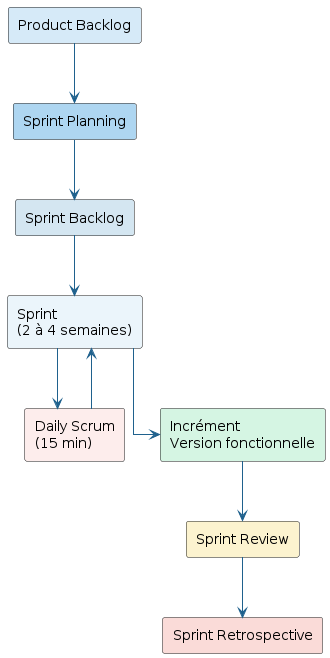
\includegraphics[width=0.5\textwidth]{Figures/Chapitre1/sprintarr.png}
\caption{Diagramme de la méthodologie Scrum}
\label{fig:ch1:scrum}
\end{figure}

\subsection{Langages de modélisation}

Pour la conception du système, le langage UML (Unified Modeling Language) est utilisé. Les principaux
diagrammes utilisés sont :

\begin{itemize}
    \item Diagramme de cas d'utilisation,
    \item Diagramme de classes,
    \item Diagramme de séquence.
\end{itemize}

Ces diagrammes permettent de représenter le fonctionnement du système de manière claire et structurée.

% ─────────────────────────────────────────────────────────────────────────────
\section*{Conclusion}

Ce chapitre a présenté le contexte général du projet et les limites du système existant. L'analyse a
montré la nécessité de développer une solution informatique adaptée. La solution proposée repose sur
une application web de gestion du service après-vente, développée selon la méthodologie Scrum. Le
chapitre suivant sera consacré à la préparation du projet et à la capture des besoins.
